\clearpage
\chapter{Integration of Transcriptomic and Proteomic data}

The work presented in this chapter was done in collaboration with Dr James Wright,
Principal Bioinformatician within the Proteomics and Mass Spectrometry unit of the
Wellcome Trust Sanger Institute and Nuno Fonseca. James performed all the
identification and quantification of the proteins, which also includes the
implementation of the new method of protein quantification presented in the
section ~\ref{subsec:newMethQuant}. Nuno performed the quality control, the mapping
and the quantification of the \dataset{Gtex} data. I have performed the quality control,
the mapping and the quantification of the \dataset{Uhlén \etal} dataset. I have also performed
all the data analysis under the supervision of Dr Alvis Brazma (EMBL-EBI) and
Dr Jyoti Choudhary (Wellcome Trust Sanger Institute).

A manuscript describing this work is being prepared with the other authors.

\section{Introduction}
\begin{comment}
%%--- \textit{or why we bother with integration?}}

    here should be explain all the reasons and the challenging of why this is
    important.
    Here some of the reasons: transcriptomics and proteomics are not the same
    range (technology bias)
    It is hard to say when it is NOT correlated if this comes from a
    technical problem or regulation.

    Workflows a lot better established in transcriptomics than proteomics
    (annotation, mapping)

\end{comment}

The core of central dogma of molecular biology --- i.e.\ one \DNA\ (coding) gene will
be transcribed as one \mRNA\ transcript and will be in turn translated in one
protein --- still holds true even though we now know the truth is not as linear as
we thought first. Many regulation processes are implied before
and after the transcription and translation steps.
In the figure \ref{dogma} which is the reconstruction by ~\cite{Crick:1958} of
what was conceived circa 1958: the solid lines present proven mode of information
transfers, the dashed ones are the ones that were postulated but still to be proven.
To update this figure to our current knowledge, the line starting from the RNA to
the DNA should be a solid one.

\begin{figure}
    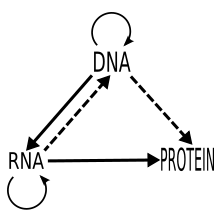
\includegraphics{integration/dogma}\centering
    \caption{\label{dogma} Central dogma of molecular biology proposed by F. Crick circa 1958}
\end{figure}

However, as we still have to prove that proteins can be produced directly
from \DNA \footnote{which seems pretty unlikely to me}, it is assumed that
each protein is created by translation, hence studying
transcriptomics and proteomics together for the same conditions should give us
insights on these regulation processes.

Whereas it was implicitly assumed for a long time that for similar conditions
there should be a proportional relationship between transcriptomics and proteomics,
many studies\
\fixme{add references, see TAC report 3}
done in cells have failed to show high correlation between the two biological layers.
From then, while there are still studies done jointly on transcriptomics and
proteomics, the focus is greater either on the presence or absence of a
protein/transcript in a specific condition or if both transcript and protein
are differential expressed between two conditions in the same way.
Nowadays, there are not many efforts to link directly their actual expression.

Previous studies did not managed to show correlation between proteomics and
transcriptomics above 0.5 (Pearson correlation coefficient).
However, while cell populations could have external factors impacting their overall
expression, tissue samples should be driven by their function.
As such we expect that what makes a liver a liver and what makes a heart a heart
would overcome most of the technical variability.

In fact, here, even though I have only access to independent data,
the average Pearson correlation is above 0.5 [min: 0.45 (Esophagus); max: 0.666 (Liver)].


In the recent past few years (2014) two large proteomics assays focusing on normal
human tissues have been released for the first time.
\fixme{add citation for Pandey and Kuster}
Until now, there was not such availability of large-scale and extensive tissues
both on transcriptomic and proteomic layer to jointly study the genes
translation into proteins across a consequent set of tissues
at the same time. Alike the \dataset{Uhlén \etal} dataset and the \dataset{Gtex}
these datasets have not the same scope of tissues. However, the overlap of
studied tissues is enough to draw an overview of the current technology.


In their review,~\cite{Uhlen:2016}, the authors outline one on-going debate
in the literature, which could be formulated whereas we should observe (or not) good
correlations between proteomic and transcriptomic data.
Indeed, first investigations found low or no correlation. More recent
studies reported improved correlations although these correlations were around
0.4 (Pearson correlation coefficient). Such discrepancies could be explained
partially by the difference of the technology for proteomic and transcriptomic
assays. Sequencing-based technologies, as \Rnaseq\, enhanced greatly the assessment
of transcripts. While true absolute quantification is not reached yet, there is
not saturation anymore or, more importantly, out-of-scope issues as they could
have been observed with microarrays. In theory, on one hand, with enough
sequencing depth, every transcript expressed in a cell or tissue could be catch
by high-throughput sequencing and in the other hand, two transcripts with different
level of expression would be differentiate  whereas they are very highly expressed
or not. If there is a difference in their level of expression, this difference
should be catch.

Unfortunately, technology on the proteomic side is not as advanced yet.
Mass spectrometry is still one of the most accurate ways to quantify the abundance
of proteins. However, often the top 25 most abundant proteins can amount for more
than 50\% of the signal collected for a sample. Therefore, the identification (and
hence quantification) of the scarcer proteins is harder.
\fixme{find reference -- ask Jyoti}

\fixme{see bottom of page2 in the paper}

\section{Data}
\label{sec:IntegrationResults}
While the \dataset{Kuster} dataset presents more tissues in common
with the Gtex and Uhlén datasets (see figures~\ref{VennTissuePandeyGtexUhlen}
and~\ref{VennTissueKusterGtexUhlen}), I had focused the study on
the \dataset{Pandey} dataset. Indeed, we managed to quantify the biggest number
of proteins in this later dataset: 10272 proteins across 24 samples for
\dataset{Pandey} versus 7223 across 24 samples for \dataset{Kuster}~\footnote{Even
if the number of samples is the same for the \dataset{Pandey} and
the \dataset{Kuster} datasets, this is purely fortuitous.}.
This has an increased importance as the study goes beyond the correlation of
proteomics and transcriptomics for a same tissue. Besides, the number of proteins
detected for a same tissue is also greater for \dataset{Pandey} as shown
in figure~\ref{KusterPandeyFQM}.
It worth noticing that even there is the same number of samples for the
\dataset{Pandey} and the \dataset{Kuster}, this is purely fortuitous.

Furthermore, all the \dataset{Pandey} data has been
collected on the same platform while the \dataset{Kuster} data has been collected on
different ones. On a side note, as each of the proteomic datasets proposes
only one sample per tissue, it is difficult to assess if the good or bad
correlation between the Kuster \etal or the Pandey \etal
proteomic data and the available transcriptomic data is due to the technology or
to the nature of the tissue.

\fixme{add Venn diagramm of Pandey, Kuster, Gtex, Uhlén shared tissues}
\begin{figure}
    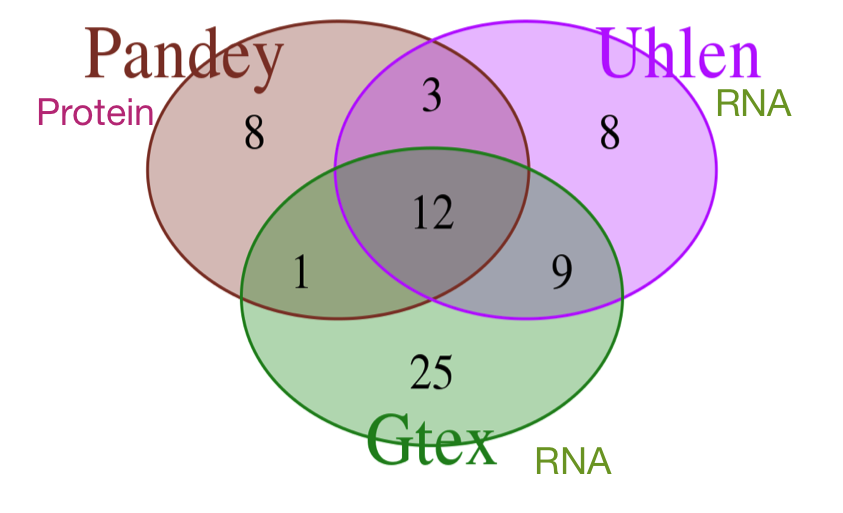
\includegraphics{integration/PandeyGtexUhlen_tissuesVenn.png}\centering
    \caption{\label{VennTissuePandeyGtexUhlen}Number of share and unique
    tissues between the proteomic dataset
    from Pandey \etal and the transcriptomic datasets (Uhlén \etal and Gtex)}
\end{figure}



\begin{figure}
    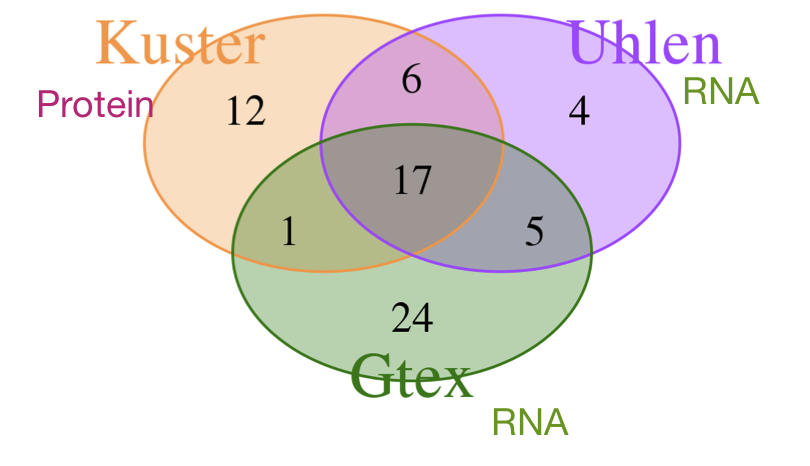
\includegraphics{integration/KusterGtexUhlen_tissuesVenn.png}\centering
    \caption{\label{VennTissueKusterGtexUhlen}Number of share and unique
    tissues between the proteomic dataset
    from Kuster \etal and the transcriptomic datasets (Uhlén \etal and Gtex)}
\end{figure}


\begin{figure}
    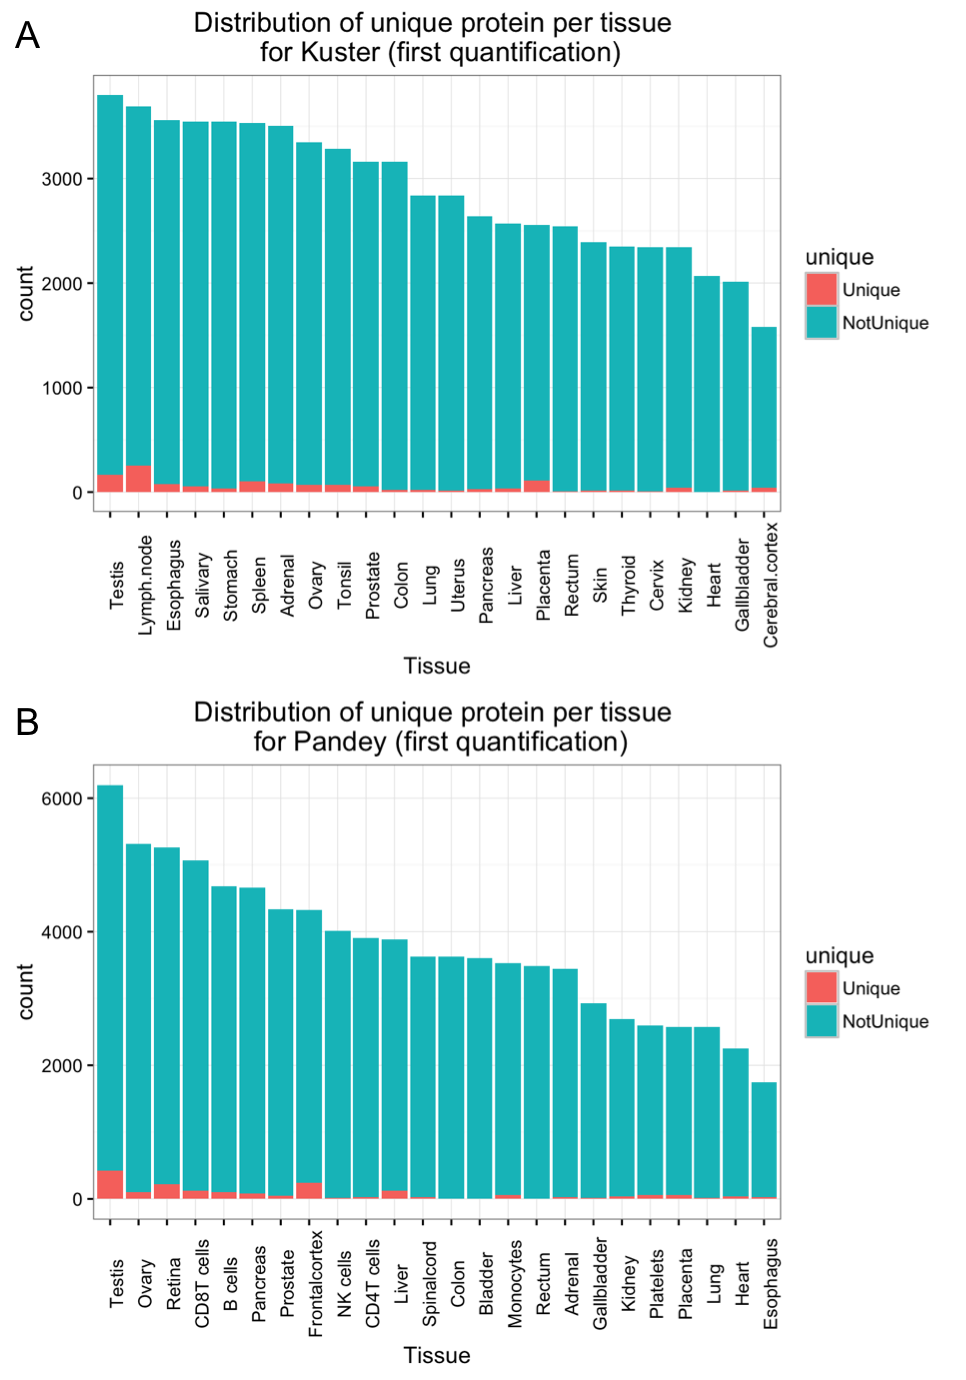
\includegraphics{integration/KusterPandeyFQM.png}\centering
    \caption{\label{KusterPandeyFQM}Distribution of proteins across the tissues
    (quantification done with the first method). Highlighted in red are the
    proteins that are found only in that
    tissue within the dataset. A) Kuster. B) Pandey.}
\end{figure}



\section{Results}
\subsection{New quantification method for the proteomic data}
\label{subsec:newMethQuant}
\textit{Quantifications performed by Dr James Wright}

At first, the quantification used for the proteomic data was following
state-of-the-art protocols with very stringent parameters:
to identify and quantify a given protein, three different unique peptides
(with a FDR < 0.01 \%) have to be mapped solely to that protein.

After discussions where we were comparing the different quantification algorithms
and methods used for \Rnaseq\ data, we decided to try a new quantification
method~\footnote{Inspired by algorithms as Cufflinks}:
the amount of proteins would take in account the unique peptides but also the
peptides that could be attributed to several proteins.
The ratio of these \emph{shared} peptides for each protein
is determined based on the amount of the other identified peptides for that protein.

Both quantification methods have been implemented by James Wright.

In the context of this work, he has quantifies about 6,400 proteins with the standard method.
The new method allowed him to quantify a bigger set of proteins: about 12,300 proteins.


I have performed the analyses presented in this chapter on both sets. As the high-level
results and conclusions are remaining the same, hereafter all the presented figures
and discussions are referring to the new quantification method. For comparison
purposes, I have produced (following the same analyses) some figures and tables
from the data quantified by the first method. Those can be found in the
appendices. To ease the comparison, their references are given in blue
(and in brackets) in the caption of the main figures.

\subsection{Independent transcriptomic and proteomic studies of normal human tissues
have good correlation}

\fixme{add figure 10 and 11 from 3rd TAC?}

%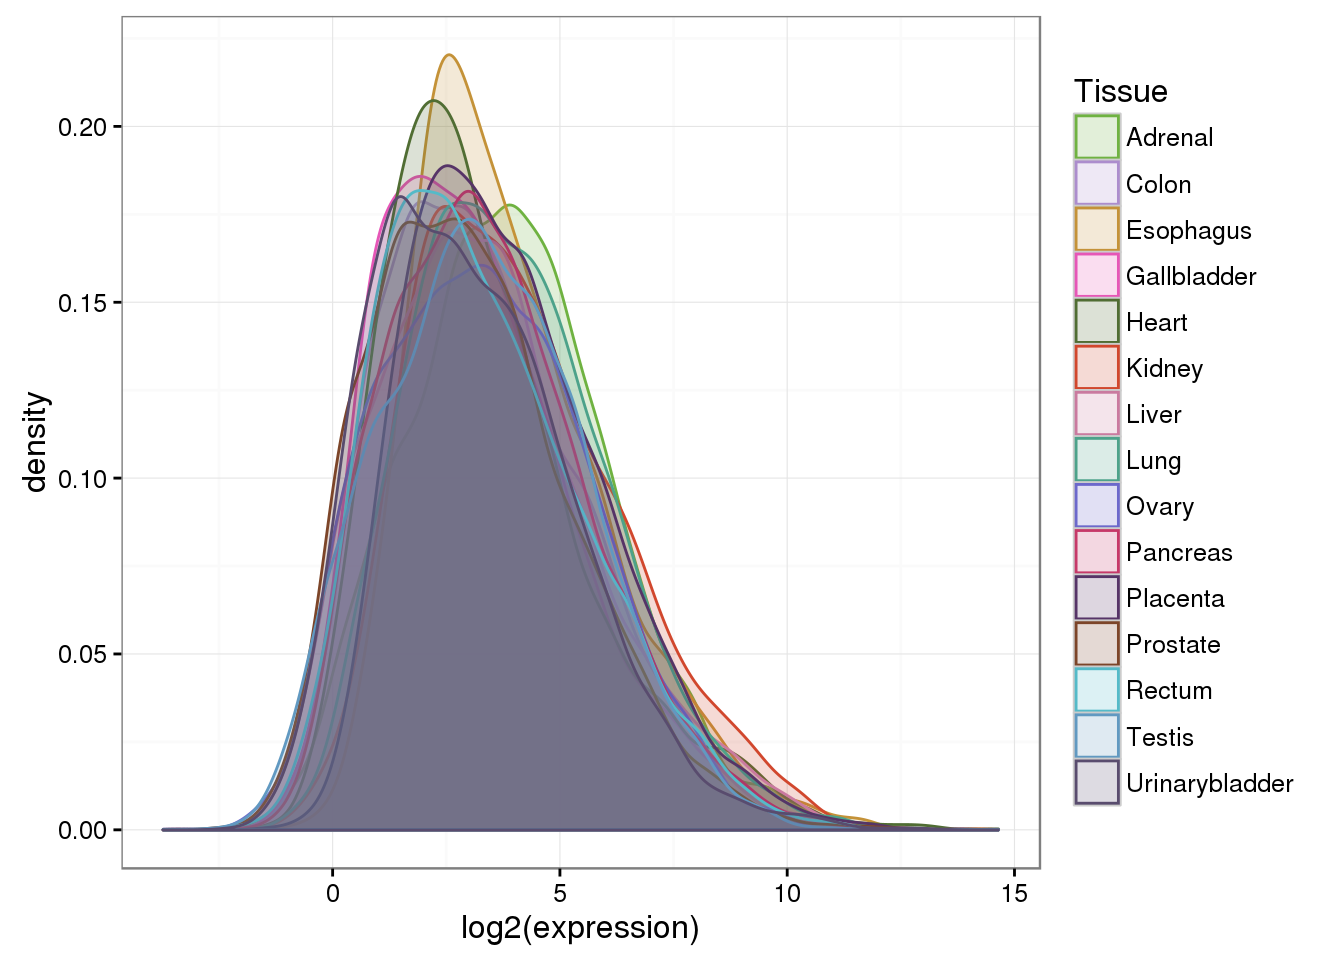
\includegraphics{integration/distributionPPKM_15Tissues_comUhlen.png}
\subsection{Distribution of expression breadth of the proteome dataset is bimodal}
\fixme{this might need to go to the previous chapter!}


Defining when a gene is expressed, ranking the expression
Tissue correlation
Tissue specific genes/proteins – how consistent they are in RNA and proteomics?
Gene correlation
Correlated and uncorrelated genes, what is specific to each group
functional groups of genes
Pseudo-gene expression



%%%%cimetiere
%%These studies however were mostly done at cell levels.
%%While the pool of protein coding transcripts is about 60 to 70 \% similar from
%%one tissue to another, the protein pool is quite different.
